% Chapter Template

\chapter{综合分离各类资源} % Main chapter title

\label{Chapter4} % Change X to a consecutive number; for referencing this chapter elsewhere, use \ref{ChapterX}

数据中心的规模日益扩张,对于内存的需求和存储的需求也越来越大。但是现阶段,数据中心的部署、执行、故障单元等都是一整台的物理服务器(monolithic server),这台服务器包含了运行一个程序所需要的全部硬件资源(CPU、内存、磁盘等)。在前面的两个章节中,我们讨论了内存分离和存储分离,这些技术能够部分提高数据中心对硬件资源的利用率,并且已经在现有的商业环境中应用。然而,这些技术仍然要部署到monolithic server上,无法解决monolithic serve本身的一些缺点,如缺乏弹性、单一硬件故障导致整台server失败等。

如果把所有的的硬件设备都组织为独立的组件,依靠网络进行通信,就可以完全打破monolithic server的体系结构,真正意义上实现硬件资源的分离,并且完全解决monolithic serve对弹性、异构性等支持不好的缺点。本章后面将以LegoOS为例,介绍这一思想。

%----------------------------------------------------------------------------------------
%	SECTION 1
%----------------------------------------------------------------------------------------

\section{背景介绍}

\subsection{硬件的发展}

近年来,网络的速度越来越快,甚至已接近内存总线速度的数量级。基于快速网络,分离的设备之间能够进行快速的通信,这使得硬件资源分离的思路成为可行。另一方面,硬件的功能和处理能力越发丰富。现代硬件可以整合大量以前由软件实现的逻辑,如控制器、网络协议栈等,这使得分离的硬件组件能够高效的进行本地管理,而不依赖CPU资源和复杂的软件逻辑。

\subsection{单一硬件资源的分离}

目前已有很多针对单一硬件资源分离的研究。例如,针对内存资源,有基于RDMA的远程换页系统INFINISWAP\parencite{gu2017efficient},可以透明的把本地计算机的内存交换到集群中另一台计算机的内存上;针对存储资源,有Flash storage disaggregation\parencite{klimovic2016flash},把闪存层从数据存储层解耦出来集中管理,使得网络中的主机可以通过统一的接口读写闪存设备。

\subsection{系统层面的分离}

???

%----------------------------------------------------------------------------------------
%	SECTION 2
%----------------------------------------------------------------------------------------

\section{相关研究}

\subsection{多机分布式计算框架}

随着需要分析处理的数据量不断增大,单台机器无法完成海量数据的计算和存储。分布式计算在此背景下产生,其主要思想是把数据和计算任务分配到多台机器上,每台机器只需承担很少的任务。这其中涉及到集群管理、消息通信、任务分发等复杂的逻辑。一些分布式计算框架,如Hadoop、Spark等的出现简化了用户的使用,用户只需编写自己的业务逻辑,底层全部交给框架处理。

这带来了很多好处,如资源被分摊到了每台机器上,单台机器的故障不会使任务彻底中断;一个良好的调度策略能够根据每台机器的性能和负载合理分配任务,尽可能最大化利用每台机器的资源;集群中的机器可以根据需要随时添加或移除;等。但是,分布式计算集群的调度单位是一整台机器,粒度很粗,无法解决单台机器内部的问题,如单台机器各硬件负载不均衡导致资源浪费。

\subsection{巨型虚拟机}

针对多机的资源利用,还有一种分布式OS的方案。其原理把每台机器的硬件资源综合在一起(例如,综合所有机器实现分布式共享内存),对外则表现为一个巨型的虚拟机。结合调度,单一的任务也能够利用到不同机器的资源,提高了硬件资源的整体利用率。但是,这种设计对节点间的通信要求较高,同时调度的策略和性能也会带来很大影响。

Amoeba\parencite{tanenbaum1991amoeba}是一个例子,它在每台机器的每个处理器核上运行一个microkernel,实现了一个共享的处理器池,为每个用户动态分配处理器资源。相比于多机分布式计算,Amoeba使资源调度的粒度减小到了进程的级别。

\subsection{弹性计算}

现在,很多云服务商都提供弹性计算服务。用户可以根据自己对资源的使用需求,灵活配置和购买。云服务商在后台管理着大量机器,将物理资源(如CPU、内存、存储、带宽等)虚拟化,并在多台机器上打通。用户对资源的使用常常是突发的,这样大多数时间物理资源是空闲的,服务商可以暂时把资源分配给其他用户。依靠资源的虚拟化和分解,实现了所有资源的按需分配,使硬件资源得到了尽可能高的利用效率。

%----------------------------------------------------------------------------------------
%	SECTION 3
%----------------------------------------------------------------------------------------

\section{案例分析:LegoOS}

\subsection{设计目标}

多年来,monolithic server一直是数据中心的部署和操作单元,但这种以单台服务器未中心的架构有几个重要的问题:
\begin{itemize}
\item 资源利用率低:由于对于同一个任务必须从同一台机器分配CPU和内存,而程序对资源的利用是不平衡的,导致硬件利用率整体不高。
\item 硬件弹性差:一旦完成单台服务器的组装,就很难添加或删除硬件组件。
\item 故障范围大:单台服务器由很多硬件组件组成,任何一个组件的损坏都会使得服务器无法工作。
\item 对异构硬件支持不好:组成单台服务器的硬件之间往往紧密的耦合,一些专用的、非传统的硬件往往难以和其他硬件组件结合。
\end{itemize}

针对以上问题,提出了一种新的硬件资源分解的架构,能够使各硬件组件完全拆分开,并在此基础上构建了LegoOS系统。

\subsection{整体架构}

\begin{figure}[h]
\centering
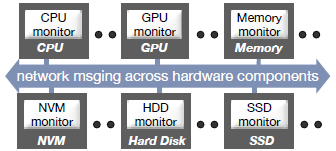
\includegraphics[scale=1.00]{Figures/legoos/splitkernel.png}
\decoRule
\caption{Splitkernel Archiecture}
\label{fig:legoos_archiecture}
\end{figure}

Splitkernel模型分解了传统操作系统的功能,并将这些功能转入松散耦合的硬件组件的监视器中。每个监视器在本地运行,管理着自己的硬件组件,并仅在需要时通过网络以显式的消息传递与其他组件通信。

LegoOS是基于splitkernel模型构建的一个专为硬件资源分解的操作系统。它将操作系统的功能分为了三类监视器:处理器监视器、内存监视器和存储监视器。除了处理器,每个硬件组件期望有一个硬件控制器,可以执行监视器的逻辑。LegoOS有全局的资源管理器GPM、GMM和GSM,用来粗粒度的分配处理器、内存和存储资源。细粒度的分配由各自的监视器决定。

\subsection{具体实现}

LegoOS在设计上针对三种硬件组件:处理器、内存、存储,分别称之为pComponent、mComponent、sComponent。在接口方面,LegoOS暴露给用户的是一组vNode。每个vNode有自己独立的IP,可以运行多个pComponent、mComponent、sComponent。LegoOS确保每个vNode的资源相互之间完全隔离。LegoOS实现了大多数的Linux system call接口,使得大多数程序可以未修改的在LegoOS的一组vNode上运行。

\subsubsection{处理器管理}

\begin{figure}[h]
\centering
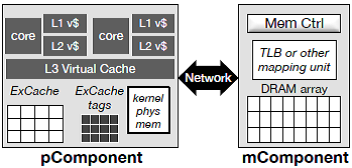
\includegraphics[scale=1.00]{Figures/legoos/1.png}
\decoRule
\caption{LegoOS pComponent and mComponent Archiecture}
\label{fig:legoos_archiecture}
\end{figure}

pComponent专门管理处理器内核。它使用了针对数据中心程序的一个简单的调度模型。每个pComponent为内核线程保留少量的核心,然后分配其他的核心给用户线程。当用户启动一个新进程时,由全局的GPM选择一个托管线程数最少的pComponent,然后这个pComponent为用户线程分配CPU核心,并且尽量减少线程调度和内核抢占以提高性能(例如,不使用中断而是用轮询处理网络请求,因为网络延迟在LegoOS中很低)。因为全局GPM的存在,调度策略的着重于最小化上下文切换的开销,而不是单个线程的核心利用率。

pComponent完全不需要地址映射,mmu和TLB等全部由mComponent维护。为了性能,在本地pComponent仍持有少量的(如4GB)内存缓存,称为ExCache,位于处理器的Last-Level Cache(LLC)之下,而剩余的大量内存通过网络从mComponent访问。每个ExCache line有一个虚拟地址的tag和两个标记位(P,R/W),由软件设置、硬件检查。当ExCache miss时,LegoOS通过网络从对应的mComponent中取回数据填入ExCache line中。ExCache miss的处理甚至可以完全由硬件实现以获得最高的效率。

ExCache冷不命中会产生很多访问mComponent的请求,带来了较大的性能开销。为此有一个简单的优化。注意到匿名内存的初始内容为零,因此可以直接在ExCache中分配这些line,直到这个ExCache line被flush,才首次发送到mComponent中。在设计上LegoOS的pComponent不共享内存,因此不会产生竞争。

\subsubsection{内存管理}

\begin{figure}[h]
\centering
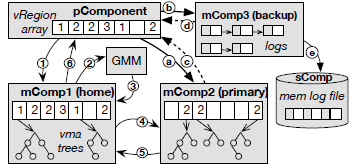
\includegraphics[scale=1.00]{Figures/legoos/2.png}
\decoRule
\caption{LegoOS Distributed Memory Management}
\label{fig:legoos_memory_management}
\end{figure}

mComponent管理虚拟内存和物理内存,包括它们的分配、回收和映射。为了最小化网络通信,这里采用了两级的内存管理。在high level,把虚拟地址空间粗粒度的划分为了固定大小的vRegions,每个已被分配的vRegion都被一个mComponent管理。在low level,mComponent记录了每个vRegion上分配给用户的vma树。一个用户进程的虚拟地址空间可以跨越多个mComponent。用户进程还有一个home mComponent,它只是记录进程的每个vRegion分别由哪个mComponnet在管理(vRegion array),以及每个vRegion内的剩余未分配空间。

当用户程序申请虚拟内存空间时,pComponent把相关的请求转发给进程的home mComponent。home mComponent会查询vRegion array,寻找一个合适的vRegion,然后把请求再转发给对应的mComponent,由它来为用户分配vma。如果可用虚拟内存空间不足,home mComponent还会向全局的内存资源管理器GMM申请一个新的vRegion并把请求转发到另一个mComponent。(实现上为了快速访问,pComponent也缓存了一份vRegion array)

考虑到内存故障的可能性与影响更大,LegoOS对mComponent提供了可靠性保证:使用primary mComponent和backup mComponent。当pComponent刷新ExCache时,消息被同时发往primary mComponnet和对应的backup mComponent。其中primary mComponent维护内存数据和元数据,backup mComponent在后台把内存操作写入由sComponent管理的append-only log中,这样可以在失败时通过log恢复内存内容。

\subsubsection{存储管理}

LegoOS在sComponent上实现存储功能。类似于NFS,存储服务器采用无状态的设计,并通过vNode抽象后暴露给用户。用户可以通过标准POSIX api操作vNode上的挂载点,从而访问存储系统。

由于sComponent的内部内存有限,LegoOS在mComponent上放置存储缓冲区。当用户通过系统调用访问文件时,抽象层把请求的文件完整路径、偏移量和大小转发给mComponent,mComponent查找缓冲区,并在需要时从sComponent获取缺失的数据以及将文件数据sync到sComponent中。

\subsection{测试评估}

由于并没有真正的资源分解硬件,硬件组件实际由服务器模拟而来,通过限制可用的资源使其符合各个componnet的设定。

\subsubsection{基准性能}

\begin{itemize}
\item 网络性能:TODO
\item 内存性能:
\item 存储性能:
\item PARSEC测试集:
\end{itemize}

\subsubsection{应用性能}

\begin{itemize}
\item TensorFlow:
\item Phoenix:
\item 多任务:
\end{itemize}

\subsubsection{故障分析}

TODO

%----------------------------------------------------------------------------------------
%	SECTION 3
%----------------------------------------------------------------------------------------

\section{本章小结}

本章主要介绍了一些综合分离各类资源的方案,如传统的多机分布式计算、巨型虚拟机,以及在云服务商大规模应用的弹性计算。这些方案从不同的技术原理、以不同的粒度实现了一定的资源分离,提高了一定的资源利用率。硬件的发展,为软件的实现提供了新的可能,使得可以跳出现有框架的限制,去尝试一些颠覆性思路。最后讨论了LegoOS,以一种全新的架构完全分离了各个硬件组件,从根本上解决了monolithic server的缺陷。
